\chapter{The Software Heritage Filesystem (SwhFS)}
\label{chp:fuse}

While the Software Heritage Vault provides a simple way to retrieve
repositories in a format suitable for existing analysis tools and workflows,
the process to do so can be tedious. This is especially true for use cases
which only need to look at specific files in the repository, in which case
users have to pay the cost of bundling, downloading and extracting the entire
repository (or directory) when only a fraction of this data is necessary.
Providing a way to work on these repositories by fetching their resources in a
\emph{lazy} way would allow researchers to quickly explore repositories and
prototype data mining tools. This kind of lazy-loading of resources over the
network can be provided at the filesystem level by \emph{virtual filesystems}.

In this chapter, we introduce the \emph{Software Heritage Filesystem
  (\SWHFS)},\footnote{\url{https://docs.softwareheritage.org/devel/swh-fuse/}}
  a user-space filesystem that gives access to the \SWH{} archive as a POSIX
  filesystem. \SWHFS{} integrates with research and development workflows by
presenting the data in the archive as regular directory trees.
Provided that a reference to the desired code can be obtained, the
corresponding file, directory, or commit can be used as if it were locally
available. More generally, \SWHFS{} offers a convenient way to explore huge
code bases~\cite{msscalar, msvfsforgit} that require significant time to be
fully retrieved over the network, large amounts of disk space, and high I/O
costs when switching branches.

\vspace{0.5cm}

This chapter is based on an article~\cite{swh-2021-swhfs}
accepted at the 43rd International Conference on Software Engineering (ICSE
2021).

% \TODO{This is a very rough copy/paste of the paper. Some parts may need
% expanding if I have enough time.}

\section{Related Work}

To the best of our knowledge \SWHFS{} is the first attempt to integrate
large-scale source code archival into development workflows via the filesystem
interface, although other VCS filesystems have been proposed in the past.

RepoFS~\cite{spinellis2019repofs} exposes a Git repository as a
FUSE~\cite{fuse, vangoor2017fuseperf} filesystem, making different trade-offs
than \SWHFS{}. RepoFS needs a \emph{local} Git repository, while \SWHFS{} loads
it lazily over the network. This makes \SWHFS{} more suitable for quick
exploration, and RepoFS more suitable for compute-intensive repository mining.

GitOD~\cite{schroeder2012gitod} and VFS for Git~\cite{msvfsforgit} expose
remote Git repositories as local filesystems, loading them lazily in order to
reduce disk and bandwidth usage for large code bases, retaining compatibility
with standard Git tools.
Scalar~\cite{msscalar} is the successor of VFS for Git and no longer provides
a virtual filesystem UX.

GitFS~\cite{presslabs-gitfs} and FigFS~\cite{grant2009figfs} also offer virtual
filesystem interfaces on top of Git. FigFS is now abandoned. GitFS is not, but
focuses on the use case of authoring new commits.

All related works reviewed thus far are Git-specific and have a
single-repository scope. \SWHFS{} is VCS-agnostic and spans the entire \SWH{}
archive, giving access to hundreds of millions of code repositories in a
unified view.

Other non-filesystem based interfaces on top of VCS repositories exist.
Gitana~\cite{cosentino2018gitana} and gitbase~\cite{sourced-gitbase} are two
such examples, providing SQL-based views onto Git repositories. While more
useful for querying and analysis, non-filesystem interfaces are less amenable
to integration with development tools.

\section{Design}

\begin{figure}
  \centering
  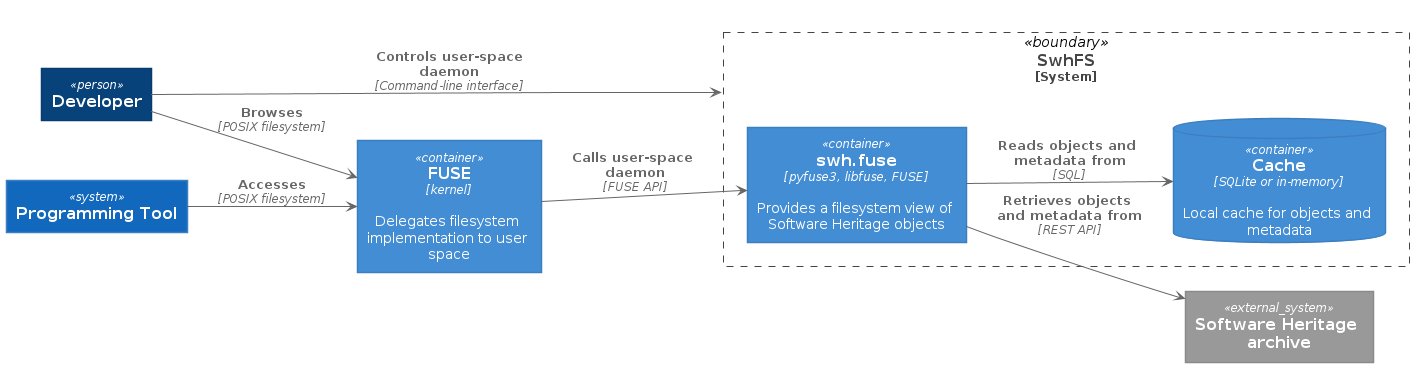
\includegraphics[width=\linewidth]{img/fuse/arch-container}
  \caption{Architecture of the Software Heritage virtual user-space filesystem
    (SwhFS)}%
  \label{fig:swhfs-arch}
\end{figure}

\Cref{fig:swhfs-arch} shows the \SWHFS{} architecture as a C4
diagram~\cite{brown2018c4}.

\subsection{Front-end: POSIX filesystem and FUSE}

Users control \SWHFS{} by starting/stopping its user-space daemon via a
convenient CLI interface. While running, \SWHFS{} provides a filesystem view of
all the source code artifacts archived by \SWH{}. This view is exposed as a
POSIX filesystem that can be browsed using file navigation tools and accessed
by programming tools like text editors, IDEs, compilers, debuggers, custom
shell scripts, etc.

According to the FUSE design~\cite{vangoor2017fuseperf}, the POSIX filesystem
interface seen by \SWHFS{} clients is implemented by the OS kernel, which
delegates decisions about the content of virtual files and directories to a
user-space daemon, communicating with it via the FUSE API~\cite{fuse}. The
\SWHFS{} daemon is implemented in the \SWHFSpy{} Python module, using the
\texttt{pyfuse3}
% ~\cite{pyfuse3}
bindings to the C FUSE API\@.

\subsection{Filesystem layout}

The filesystem layout implemented by \SWHFSpy{} consists of (1) a set of entry
points and (2) filesystem representations of \SWH{} objects. \emph{Entry points}
are located just below the \SWHFS{} mount point; most notably \texttt{archive/}
allows browsing the \SWH{} archive by known SWHIDs while \texttt{origin/} allows
doing so by the URLs of archived projects (see \cref{sec:fuse-walkthrough}
for examples).
% For instance, \lstinline{cd archive/swh:1:dir:c6f0[..]900f/} will enter the
% archived source tree corresponding to the given SWHID.

\emph{Filesystem representations} of \SWH{} objects depend on the object type:
% (source code files and directories, commits, releases, etc.). As a first
% approximation:
\begin{itemize}

\item \emph{Source code files} (SWHID type: \texttt{cnt}) are represented as
  regular POSIX files; everything else is mapped to directories.

\item \emph{Source code directories} (\texttt{dir} type) as directories whose
  content matches what was archived.

\item \emph{Commits and releases} (\texttt{rev} and \texttt{rel}) as
  directories containing a \texttt{root} sub-directory pointing to the source
  code tree plus auxiliary files containing metadata such as commit message and
  ancestry, timestamps, author information, etc.

\item \emph{Repository snapshots} (\texttt{snp}) as directories containing one
  entry for each repository branch (\texttt{master}, \texttt{v1.0},
  \texttt{bug-6531}, etc.), each pointing to the filesystem representation of
  the corresponding commit or release.

\end{itemize}

Relationships between accessed archived objects are represented using symbolic
links. For instance, the source tree of a commit object
\texttt{archive/swh:1:rev:…/root} is a symbolic link to a directory object
located under \texttt{archive/}, e.g., \texttt{"->~../../swh:1:dir:…"}. This
approach avoids duplications in the virtual filesystem, reifying the sharing of
Merkle structures on disk.

The walkthrough of \cref{sec:fuse-walkthrough} presents additional details
about the \SWHFS{} filesystem layout. A full layout specification is included
with \SWHFS{} documentation.
% it's in the intro already:
% \footnote{\url{https://docs.softwareheritage.org/devel/swh-fuse/}}


\subsection{Backend: a \SWH{} $\leftrightarrow$ FUSE adapter}

\SWHFSpy{} is an adapter between the \SWH{} REST
API\footnote{\url{https://archive.softwareheritage.org/api/}} (SWH API) and the
FUSE API\@. When filesystem entities that represent archived objects are
accessed, \SWHFSpy{} uses the SWH API to retrieve data and metadata about them.
Obtained results are then used to assemble the expected filesystem layout and
return it to the kernel via the FUSE API\@.

For example, when a source tree object is listed using
\mintinline{c}{readdir()}, \SWHFS{} invokes the \texttt{/directory} endpoint of
the \SWH{} API and return to the kernel its directory entries using a lazy
iterator; when a source code file is \mintinline{c}{open()}-ed,
\texttt{/content/raw} is called and byte chunks of the retrieved blob are
returned to the kernel piecemeal.

As part of adaptation, \SWHFSpy{} takes care and abstracts over details such as
pagination, encoding issues, inode and file description allocation, etc.


\subsection{Performance optimizations}

Remote filesystems can be notoriously painful to use, on account of network
overhead.  To make things worse for \SWHFS, the backend technology stack (REST
APIs and long-term archival storage) was not designed with filesystem-level
performances in mind. In order to make it fast enough for practical use,
\SWHFS{} implements several optimizations.


\paragraph*{Caching}

Several \emph{on-disk caches} are stored in SQLite databases to avoid repeating
remote API calls.
% ~\cite{owens2006sqlitebook}
The \emph{blob cache} stores raw source code file contents. The \emph{metadata
  cache} stores the metadata of any kind of object which has already been
  looked up. Using these two caches it is possible to navigate any part of the
  \SWH{} archive that has been accessed in the past, even while disconnected
  from the network.

Merkle properties and the read-only nature of \SWHFS{} make cache invalidation
unnecessary, as no cached object can ever change. The option of purging objects
from these caches also remains available.

\emph{In-memory caching} is used for directories, as is typical in most
filesystems. The \emph{direntry cache} maps directories to their entries, so
that frequently accessed directories can be listed without even incurring
SQLite query costs.


% THIS WILL BE INTRODUCED LATER IN THE THESIS. Can't talk about this here.
%
% \paragraph*{Compressed in-memory graph representation}
% 
% When accessing commits and release objects, developers often need to quickly
% explore their commit history, \emph{à la} \texttt{git} \texttt{log}. Exploring
% commit histories via the core SWH API would be too slow for that, as one HTTP
% call per commit is needed, times tens or hundreds of thousand commits for large
% repositories, with no parallelization opportunity, given that commit
% identifiers are discovered incrementally.
% 
% To address this issue we built upon
% \texttt{swh-graph},\footnote{\url{https://docs.softwareheritage.org/devel/swh-graph/}}
% a compressed in-memory representation of the \SWH{} archive, obtained applying
% webgraph compression techniques~\cite{saner-2020-swh-graph}. The compressed
% structure of the global VCS graph comprising 17\,B nodes and 200\,B edges
% fits in $\approx$100\,GiB of RAM and can be visited with amortized traversal
% cost close to a single memory access per traversed edge.
% 
% We have extended the SWH API to expose the \texttt{swh-graph} graph traversal
% API\@. For commit objects, \SWHFS{} invokes it to perform a graph visit of all
% reachable commits and then populate several \emph{history summary views} which
% are available under the \texttt{history/by-date/}, \texttt{history/by-hash/},
% and \texttt{history/by-page/} directories (see \cref{sec:fuse-walkthrough}
% for details). Even for huge repositories like the Linux kernel, retrieving the
% full commit history (as a list of SWHIDs) requires just a few tens of seconds,
% including network transfer.


\paragraph*{Asynchronicity}

In order to maximize I/O throughput, \SWHFS{} is implemented in asynchronous
style:
% (using asyncio~\cite{hunt2019asyncio}),
all blocking operations yield control to other coroutines instead of blocking.
%
Additionally, SWH API calls are delegated to a shared thread pool that can keep
persistent HTTP connections to the remote API backend, rather than establishing
new ones at each call.


\section{Walkthrough}
\label{sec:fuse-walkthrough}

This section shows how to use \SWHFS{} via concrete examples. A screencast video
is available online at \url{https://dx.doi.org/10.5281/zenodo.4531411}.

\paragraph{Installation}

\SWHFS{} is implemented in Python, released under the GPL3 license, and
distributed via PyPI.
% as \SWHFSpy.\footnote{\url{https://pypi.org/project/swh.fuse/}}
It can be installed from there running \mintinline{bash}{pip install swh.fuse}.

\SWHFS{} development happens on the \SWH{}
forge,\footnote{\url{https://forge.softwareheritage.org/source/swh-fuse/}}
where issues and patches can be submitted.

\paragraph{Setup and teardown}

Like with any filesystems, \SWHFS{} must be ``mounted'' before use and
``unmounted'' afterwards. Users should first mount the \SWH{} archive as a whole
and then browse archived objects looking up their SWHIDs below the
\texttt{archive/} entry-point. To mount the Software Heritage archive, use the
\texttt{swh fs mount} command:

\begin{minted}{console}
$ mkdir swhfs
$ swh fs mount swhfs/  # mount the archive
$ ls -F swhfs/  # list entry points
archive/  cache/  origin/  README
\end{minted}

By default \SWHFS{} daemonizes in background and logs to syslog; it can be kept
in foreground, logging to the console, by passing \texttt{-f/--foreground} to
\texttt{mount}.

To unmount \SWHFS{} use \texttt{swh fs umount PATH}. Note that, since
\SWHFS{}
is a \emph{user-space} filesystem, (un)mounting are not privileged operations,
any user can do it.

The configuration file \texttt{\~{}/.swh/config/global.yml} is read if
present. Its main use case is inserting a per-user authentication token for the
SWH API, which might be needed in case of heavy use to bypass the default API
rate limit.


\paragraph{Source code browsing}

Here is a \SWHFS{} Hello World:

\begin{minted}{console}
$ cd swhfs/
$ cat archive/swh:1:cnt:c839dea9e8e6f0528b468214348fee8669b305b2
\end{minted}
\inputminted{c}{codesamples/swh-fuse/hello.c}

Given the SWHID of a source code file, we can directly access it via the
filesystem. We can do the same with entire source code directories. Here is the
historical Apollo 11 source code, where we can find interesting comments about
the antenna during landing:

\begin{minted}{console}
$ cd archive/swh:1:dir:1fee702c7e6d14395bbf5ac3598e73bcbf97b030
$ ls | wc -l
127
$ grep -i antenna THE_LUNAR_LANDING.s | cut -f 5
# IS THE LR ANTENNA IN POSITION 1 YET
# BRANCH IF ANTENNA ALREADY IN POSITION 1
\end{minted}

We can checkout the commit of a more modern codebase, like jQuery, and count
its JavaScript lines of code (SLOC):

\begin{minted}{console}
$ cd archive/swh:1:rev:9d76c0b163675505d1a901e5fe5249a2c55609bc
$ ls -F
history/  meta.json@  parent@  parents/  root@
$ find root/src/ -type f -name '*.js' | xargs cat | wc -l
10136
\end{minted}

\paragraph{Commit history browsing}

\texttt{meta.json} contains complete commit metadata, e.g.:

\begin{minted}{console}
$ jq .author.name,.date,.message meta.json
"Michal Golebiowski-Owczarek"
"2020-03-02T23:02:42+01:00"
"Prevent collision with Object.prototype ..."
\end{minted}

Commit history can be browsed commit-by-commit digging into \texttt{parent(s)/}
directories or, more efficiently, using the history summaries located under
\texttt{history/}:

\begin{minted}{console}
$ ls -f history/by-page/000/ | wc -l
6469
$ ls -f history/by-page/000/ | head -n 2
swh:1:rev:358b769a00c3a09a...
swh:1:rev:4a7fc8544e2020c7...
\end{minted}

The jQuery commit at hand is preceded by \num{6469} commits, which can be
listed in ``\texttt{git log}'' order via the \texttt{by-page} view. The
\texttt{by-hash} and \texttt{by-date} views, inspired by
RepoFS~\cite{spinellis2019repofs}, list commits sharded by commit identifier
and timestamp:

\begin{minted}{console}
$ ls history/by-hash/00/ | head -n 1
swh:1:rev:0018f7700bf8004d...
$ ls -F history/by-date/
2006/  2007/  2008/  ...  2018/  2019/  2020/
$ ls -f history/by-date/2020/01/08/
swh:1:rev:437f389a24a6bef...
$ jq .date history/by-date/2020/01/08/*/meta.json
"2020-01-08T00:35:55+01:00"
\end{minted}

Note that to populate the \texttt{by-date} view, metadata about all commits in
the history are needed. To avoid blocking, metadata are retrieved asynchronously
in the background, populating the view incrementally. The hidden
\texttt{by-date/.status} file provides a progress report and is removed upon
completion.


\paragraph{Repository snapshots and branches}

Snapshot objects keep track of where each branch and release (or ``tag'')
pointed to at archival time. Here is an example with the Unix history
repository~\cite{SpinellisUnix2017}, which uses historical Unix releases as
nested branch names:

\begin{minted}{console}
$ cd archive/swh:1:snp:2ca5d6eff8f04a671c0d5b13646cede522c64b7d/refs/heads
$ ls -f | wc -l ; ls -f | grep Bell
40
Bell-32V-Snapshot-Development
Bell-Release
$ cd Bell-Release
$ jq .message,.date meta.json
"Bell 32V release ..."
"1979-05-02T23:26:55-05:00"
$ grep core root/usr/src/games/fortune.c
      printf("Memory fault -- core dumped\n");
\end{minted}

Two of the 40 top-level branches correspond to Bell Labs releases. We can dig
into the UNIX/32V \texttt{fortune} implementation instantly, without having to
clone a 1.6\,GiB repository.


\paragraph{Software origins}

Software can also be explored by the URL it was archived from, using the
\texttt{origin/} entry point:

\begin{minted}{console}
$ cd origin/
$ cd https%3A%2F%2Fgithub.com%2Ftorvalds%2Flinux
$ ls
2015-07-09/  2016-02-23/  2016-03-28/  ...
$ ls -F 2015-07-09/
meta.json  snapshot@
\end{minted}

we can see a list of all archival crawls of the Linux kernel repository made by
Software Heritage, and then navigate to the state of the repository as it was
in 2015 (as a snapshot object). Note that one needs to use the exact origin URL
and percent-encode it. To help with that, the companion \texttt{swh web search}
CLI tool is available:

\begin{minted}{console}
$ swh web search "torvalds linux" --limit 1 --url-encode | cut -f1
https%3A%2F%2Fgithub.com%2Ftorvalds%2Flinux
\end{minted}


\section{Discussion}

\SWHFS{} provides numerous improvements in archive data accessibility.
It considerably reduces the friction of accessing various software artifacts as
it does not require any up-front setup to navigate any software artifact once
the virtual filesystem has been mounted. This is very useful for prototyping
experiments, as it allows researchers to use software mining tools as if the
source code files were on their local computers. When using a filesystem interface,
existing POSIX tools and coreutils can be used to easily select files on which
to run analyses (\mintinline{console}{find}, \mintinline{console}{ls **/*.c},
etc.).

Because each file is fetched lazily when its contents are accessed, this
reduces the total size of the objects retrieved from the archive, in contrast
to the Vault which always bundles an entire subgraph and all the objects it
contains, even when they are not necessary for the analysis. This makes
\SWHFS{} an efficient way to run experiments that only access a small number of
specific files in a repository, e.g., license or README files.
Moreover, the use of symbolic links to implement sharing relationships between
the software artifacts materializes the DAG in a way that can be studied
practically: it is easy to check whether two artifacts are the same by
checking whether their symbolic link resolves to the same filesystem node. This
makes it possible to implement graph traversal algorithms directly at the
filesystem level.

However, \SWHFS{} has a few important limitations that makes it generally
unsuitable for large-scale software mining. First, it is not optimized for
heavy workloads, as its primarily goal was to target small experiments and
localized analyses. The software components of \SWHFS{} (the SQLite cache, the
HTTP library, etc.) were not designed to handle large-scale analyses, high
parallelism and data intensive tasks. In general, while user-space filesystems
based on FUSE can sometimes reach performance reasonably close to kernel-level
filesystems, they require a particular attention on optimization and some
workloads are unfriendly even when optimized~\cite{vangoor2017fuseperf}.

While there is always room for performance improvements, another important
issue that makes \SWHFS{} often unsuitable for large-scale mining is the lack of
entry-points to find the relevant artifacts. The virtual filesystem makes
it easy to find all the Python files in a single repository, for instance,
but there is no easy way to find all the files or revisions matching a certain
pattern in the entire archive. As described in
\cref{sec:mining-selection-criteria}, software mining studies are often
designed to be run on arbitrary artifacts matching certain criteria. \SWHFS{}
does not provide a way to iterate on these artifacts, as its primary function
is to list the descendants of a given node in the software graph.

\bigskip

The Vault and \SWHFS{} provide two different ways to perform studies on
individual artifacts and their descendants, and thus make the data corpus
available for small to medium-scale studies ($\approx$ tens of thousands of
repositories) assuming researchers have pre-established a list of repositories
of interest for their study.
The next logical step is to explore ways to efficiently select massive
quantities of software artifacts on more fine-grained criteria, and
run analyses for larger workloads, up to the size of the entire archive.
